\documentclass[a4paper,12pt]{report}

\usepackage{alltt, fancyvrb, url}
\usepackage{graphicx}
\usepackage[utf8]{inputenc}
\usepackage{float}
\usepackage{hyperref}

\hypersetup{
    colorlinks=true,
    linkcolor=black,
    filecolor=magenta,      
    urlcolor=blue,
    pdfpagemode=FullScreen,
    }

\title{Assignment 02 - \\``Smart Waste Disposal System''\\
    \large ``Embedded Systems e Internet of Things'' final report}

\author{Lorenzo Cinelli}
\date{\today}

\begin{document}

\maketitle

\tableofcontents

\chapter{Analysis}

    \section{Description}

        The system required is a smart waste disposal system for - potentially dangerous - liquids. It has to be composed by a container having some sensors to check the temperature of the waste and the filling level. It has also two leds and a screen to signal if the user can spill the waste or not in case of some behavior. To spill the waste there is a door controlled by two buttons - one to open it and one to close it. 
        There is also an operator dashboard where operators can handle problems, empty the container or consult information about the container. If no user is spilling waste the system waits a timeout and then goes in \textit{sleep mode}. 

        \begin{figure}[H]
        	\centering{}
        	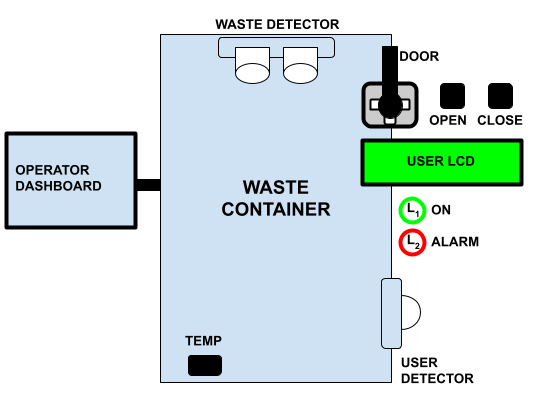
\includegraphics[width=250pt]{img/Assignment-02_SWDS-Domain.png}
        	\caption{Smart Waste Disposal System}
        	\label{img:system}
        \end{figure}

    \section{Domain Model}

    \section{Requirements}

\chapter{Design}

\chapter{Develop}

\appendix
\chapter{User Guide}

\end{document}